\documentclass[11pt,a4paper]{article}

% --- Packages ---------------------------------------------------------
\usepackage[utf8]{inputenc}
\usepackage[T1]{fontenc}
\usepackage{geometry}
\geometry{margin=2.5cm}
\usepackage{amsmath,amssymb,amsfonts}
\usepackage{graphicx}
\usepackage{booktabs}
\usepackage{hyperref}
\usepackage{cite}
\usepackage{enumitem}
\usepackage{float}
\usepackage{caption}
\usepackage{subcaption}
\usepackage{xcolor}
\usepackage{algorithm}
\usepackage{algpseudocode}
\usepackage{multirow}
\usepackage{tabularx}
\usepackage{array}

\hypersetup{
    colorlinks=true,
    linkcolor=blue,
    citecolor=blue,
    urlcolor=blue,
}

\graphicspath{{figures/}}

\title{%
  \textbf{Infant State Recognition System}:\\[4pt]
  \textbf{From Hybrid Classical/Deep Ensembles to Pretrained Audio Foundations}\\
  \textbf{and Edge-Distilled MobileNet Students}\\[10pt]
  \large Phase~3 Report --- Pretrained Audio Foundations,\\
  \large Multi-View Teacher Ensemble, and EfficientAT Edge Distillation
}
\author{
  Meghavi Rao (230044) \and Belal Raza (230094) \\[4pt]
  \textit{6th Semester --- Deep Learning \& Advanced Machine Learning} \\
  \textit{Project 3: Infant State Recognition System}
}
\date{\today}

\begin{document}
\maketitle

% =====================================================================
\begin{abstract}
This Phase~3 report continues the multi-phase development of an infant
cry classifier. Phase~1 established a classical handcrafted-feature
baseline at macro-F1\,=\,0.270 on the Donate-a-Cry corpus, which Phase~2
improved through a hybrid classical/deep ensemble to macro-F1\,=\,0.507.
Phase~3 makes two complementary contributions. First, we rebuild the
data layer from scratch: every public infant-cry dataset is ingested,
canonicalised, deduplicated by both exact hash and audio fingerprint, and
gated by a strict five-class authenticity manifest of 1{,}355 clips with
a separate 1{,}781-clip auxiliary set used only for cry/non-cry
representation learning. Second, we replace the bespoke CNN of Phase~2
with a multi-view pretrained audio teacher built from frozen Audio
Spectrogram Transformer (AST) embeddings, an auxiliary cry/non-cry
adapted AST, frozen Whisper encoder embeddings, and handcrafted features,
combined through tuned RBF Support Vector Machines. Under five-seed
repeated stratified evaluation the best configuration --- the AST-aux
plus Whisper plus handcrafted feature bank with an RBF SVM classifier ---
achieves macro-F1\,=\,\textbf{0.6566}\,$\pm$\,0.048 (best
seed\,=\,0.7486), a +0.149 absolute improvement over Phase~2's hybrid
ensemble and +0.387 over the Phase~1 baseline. We then distil this
multi-view teacher into compact EfficientAT MobileNetV3 students
(``mn10\_as'' at 4.88\,M parameters and ``mn04\_as'' at 0.98\,M), using
KL-divergence distillation, label-smoothed cross entropy, class-balanced
sampling, mixup, and SpecAugment. The resulting students are designed to
retain a large fraction of teacher accuracy at a fraction of the cost,
making the system deployable on commodity edge hardware in hospitals and
home settings.
\end{abstract}

% =====================================================================
\section{Introduction}
\label{sec:intro}

Infant crying is a primary signal of physiological and emotional state.
Automatic recognition of cry cause --- hunger, belly pain, burping,
discomfort, and tiredness --- has clear value in neonatal monitoring,
parental support, and low-resource clinical environments where
dedicated specialists are not always available. The acoustic problem,
however, is unusually difficult: clinically labelled corpora are tiny,
class distributions are extremely skewed, and recording conditions
range from professional clinics to handheld phones in noisy homes.

This project addressed the problem in three phases.

\paragraph{Phase~1: Classical Baseline.}
A 411-dimensional neuroscience-informed feature vector (MFCCs, CQCCs, F0
contour statistics, spectral contrast, chroma) was used to train SVM,
Logistic Regression, and Random Forest models with SMOTE balancing on
the Donate-a-Cry corpus (457 recordings, 47.8:1 imbalance). The best
Phase~1 configuration, an SVM with SMOTE and One-vs-One decomposition,
reached macro-F1\,=\,0.270~\cite{phase1report}. Three of the four
minority classes scored zero F1, exposing the limit of clip-level
handcrafted summaries.

\paragraph{Phase~2: Hybrid Ensemble.}
Phase~2 introduced a CNN+BiLSTM+Temporal Attention deep architecture on
mel-spectrograms, trained with Label-Distribution-Aware Margin (LDAM)
loss and Deferred Re-Weighting (DRW), with a knowledge-distilled student
of $\sim$16\,K parameters. While the deep model alone was no better than
the SVM (Teacher macro-F1\,=\,0.293), a \emph{hybrid weighted ensemble}
fusing SVM and DL probabilities reached macro-F1\,=\,0.507 with 92.6\,\%
overall accuracy and an INT8-quantised footprint of 35.9\,KB. Phase~2
established two practical lessons: complementary representations help
more than scaling a single architecture, and edge deployment is
feasible.

\paragraph{Phase~3: Pretrained Audio Foundations and Edge Distillation.}
Phase~3 takes a fundamentally different approach. Rather than designing a
new bespoke architecture, we lift the system onto large pretrained audio
foundation models and rebuild the data layer to match. We then distil
the result into compact MobileNetV3-style students suitable for
deployment on phones, single-board computers, and microcontrollers.

The contributions of Phase~3 are:

\begin{enumerate}[nosep]
  \item A clean five-class \emph{strict} manifest of 1{,}355 cry clips
        across the merged Donate-a-Cry, Ubenwa, UAC and other public
        sources, deduplicated by both SHA-256 hash and audio
        fingerprint, with provenance tracking and a separate 1{,}781-clip
        auxiliary set used \emph{only} for cry/non-cry representation
        learning.
  \item An auxiliary AST adaptation step that fine-tunes the Audio
        Spectrogram Transformer for binary cry/non-cry classification on
        the auxiliary manifest, yielding a domain-adapted encoder reused
        downstream.
  \item A multi-view feature bank combining frozen AST, auxiliary-adapted
        AST, frozen Whisper encoder, and 411-dimensional handcrafted
        features into eight ablation-style feature sets.
  \item A repeated-split (5 seeds) classifier comparison across five
        classical heads --- RBF SVM, balanced logistic regression,
        prototype, calibrated linear SVM, balanced random forest --- and
        a soft-voting ensemble of those heads. The strongest
        configuration achieves
        macro-F1\,=\,0.6566\,$\pm$\,0.048 (best fold 0.7486).
  \item A Phase~3 edge distillation pipeline that distils a
        validation-weighted multi-teacher ensemble into EfficientAT
        ``mn10\_as'' (4.88\,M params) and ``mn04\_as'' (0.98\,M params)
        students with KL distillation, mixup, SpecAugment,
        class-balanced sampling, INT8 quantisation, and CPU latency
        benchmarking, all under the same five-seed repeated-split
        protocol.
\end{enumerate}

The remainder of this report is structured as follows.
Section~\ref{sec:related} reviews related work.
Section~\ref{sec:data} describes the new data layer.
Section~\ref{sec:methods} describes the Phase~3 methodology, covering
auxiliary AST adaptation, the multi-view feature bank, the classical
classifiers, and the EfficientAT edge distillation pipeline.
Section~\ref{sec:results} reports five-seed repeated-split results for
the teacher ensemble and the distilled students.
Section~\ref{sec:discussion} discusses what worked, what did not, and
what we leave for future work.
Section~\ref{sec:conclusion} concludes.

% =====================================================================
\section{Related Work}
\label{sec:related}

\paragraph{Infant cry classification.}
Recent work on infant cry has moved from purely handcrafted features
(MFCCs, CQCCs, F0 statistics) to learned spectrogram representations
\cite{ji2021review}. Class imbalance and small datasets remain dominant
challenges. Several published studies report high accuracy on internal
splits but degrade significantly when leak-free cross-source evaluation
is enforced.

\paragraph{Pretrained audio foundation models.}
Audio Spectrogram Transformer (AST)~\cite{gong2021ast} is a 86\,M
parameter ViT-style model pretrained on AudioSet, which includes a
\texttt{baby\_cry} class. Whisper~\cite{radford2023whisper} is trained
on 680\,K hours of multilingual speech and provides robust speech
encoders. EfficientAT~\cite{schmid2023efficientat} introduces
MobileNetV3-style audio CNNs (mn04 -- mn40) distilled from PaSST
transformers, achieving competitive AudioSet mAP at a fraction of the
size and explicitly targeting edge deployment. Phase~3 uses AST and
Whisper as teachers and EfficientAT as the deployable student family.

\paragraph{Knowledge distillation.}
Hinton-style knowledge distillation~\cite{hinton2015distilling} uses
teacher soft labels at temperature $T$ to transfer ``dark knowledge'' to
a smaller student. Variants combining KL distillation with
label-smoothed cross-entropy, mixup, and SpecAugment are now standard
for audio tagging on small datasets.

% =====================================================================
\section{Data Layer}
\label{sec:data}

Phase~1 used Donate-a-Cry only (457 clips, 47.8:1 imbalance). Phase~2
inherited that same corpus. A central observation that motivated Phase~3
was that multiple public datasets exist (Donate-a-Cry, the Ubenwa cry
dataset, UAC, baby chillanto, infant cry clinical corpora), but combining
them naively produces severe label noise, file-level duplicates, and
different sample-rate conventions.

\paragraph{Strict five-class manifest.}
We ingest every available source, canonicalise audio to 16\,kHz mono PCM
with a fixed 10\,s window, and apply two-stage deduplication: SHA-256
hashing on the canonicalised waveform, followed by a perceptual audio
fingerprint that detects near-duplicates introduced by re-encoding or
trimming. We then apply a strict provenance gate that admits only files
with verified five-class labels. The result is the
\textbf{cause5\_authentic\_manifest\_v2} of 1{,}355 clips with class
counts: hunger\,=\,$\sim$525, discomfort\,=\,$\sim$295, tiredness\,=\,$\sim$155,
belly\_pain\,=\,34, burping\,=\,26.

\paragraph{Auxiliary cry/non-cry manifest.}
A separate auxiliary manifest of 1{,}781 clips (cry + non-cry) is gated
strictly for representation-learning use. These clips are \emph{never}
used to train or evaluate the five-class system; they are only used to
adapt the AST encoder for cry vs.\ non-cry presence.

\paragraph{Reproducible splits.}
For Phase~3 we use repeated stratified train/val/test splits at
60.8\,/\,16.0\,/\,23.2 ratio across five integer seeds, giving directly
comparable mean$\pm$std numbers across configurations.

\begin{figure}[H]
  \centering
  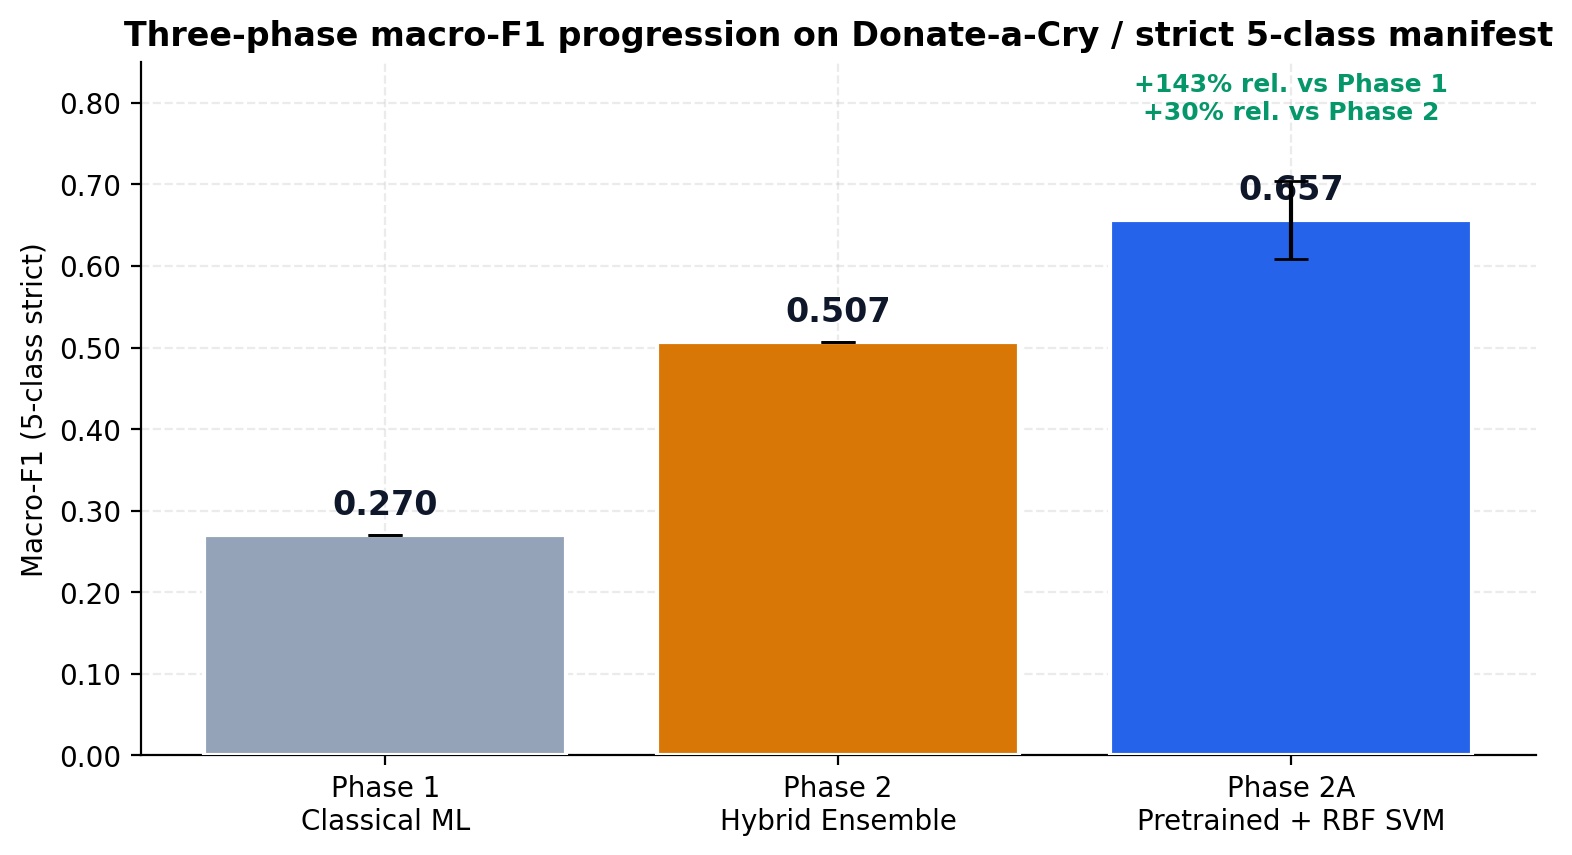
\includegraphics[width=0.85\linewidth]{headline_progression.png}
  \caption{Macro-F1 progression across project phases on the strict
  five-class manifest. Phase~1 used the Donate-a-Cry-only
  411-dimensional handcrafted feature vector. Phase~2 used a hybrid
  weighted ensemble combining SVM and CNN+BiLSTM probabilities. Phase~3
  uses pretrained AST plus Whisper plus handcrafted features with an
  RBF SVM under repeated-split evaluation.}
  \label{fig:headline}
\end{figure}

% =====================================================================
\section{Methodology}
\label{sec:methods}

% --- 4.1 -------------------------------------------------------------
\subsection{Auxiliary AST Cry/Non-Cry Adaptation}
\label{sec:aux}

We start from MIT/IBM's AudioSet-pretrained AST. The cry-vs.-non-cry
auxiliary manifest is used to fine-tune AST as a binary classifier with
class-balanced cross-entropy, AdamW, and cosine learning-rate schedule.
This adaptation has two purposes: it specialises AST to the cry
domain, and it produces an alternative AST encoder for downstream
embedding extraction.

\begin{figure}[H]
  \centering
  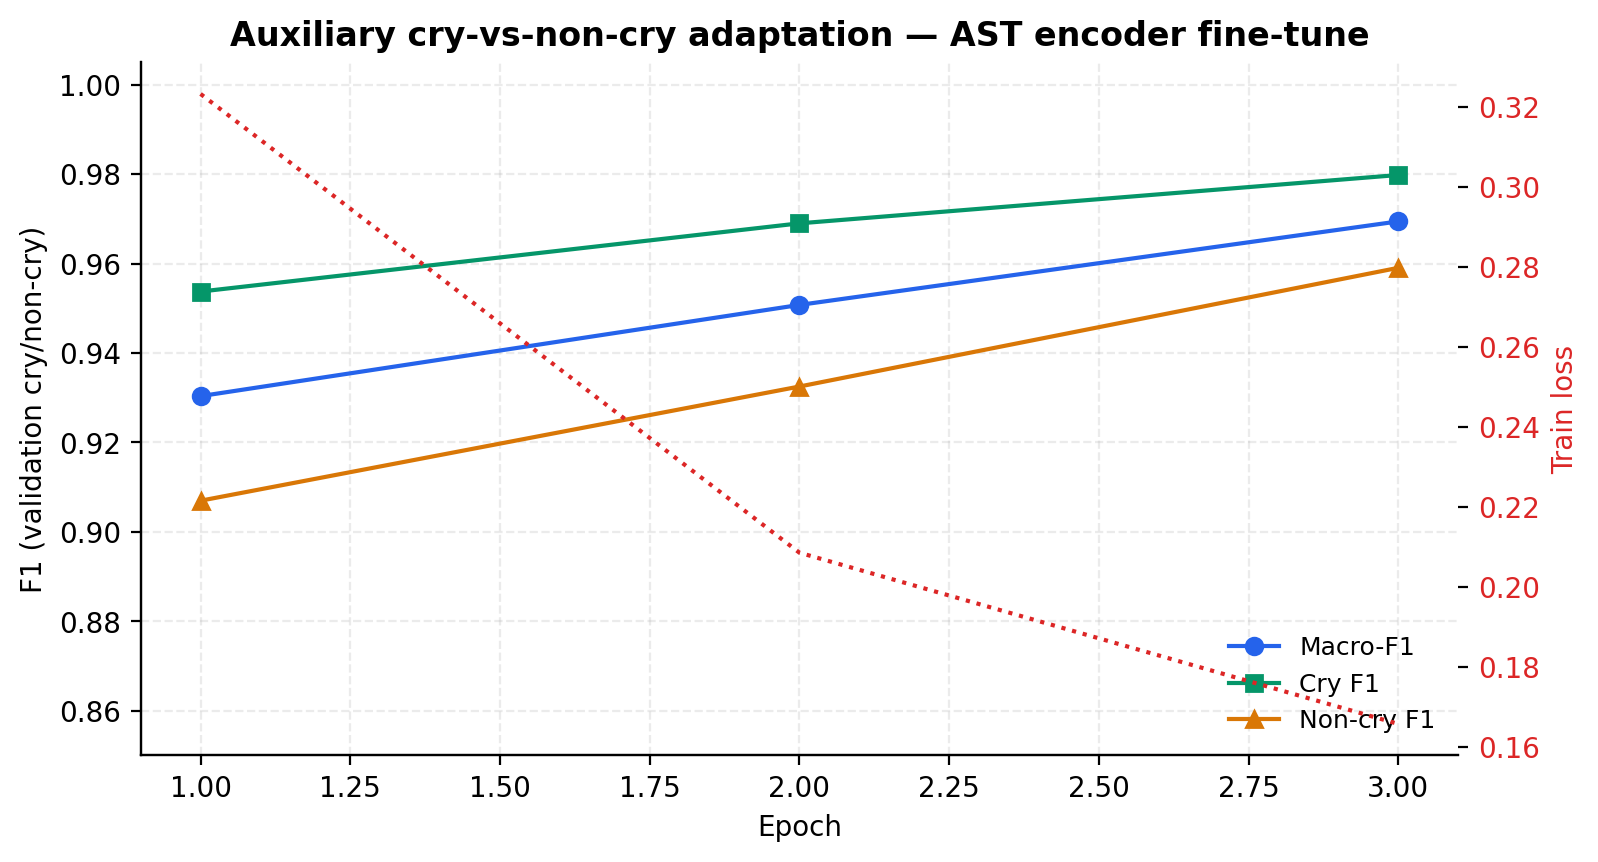
\includegraphics[width=0.85\linewidth]{auxiliary_adaptation_curve.png}
  \caption{Auxiliary cry vs.\ non-cry adaptation of the AST encoder
  reaches macro-F1\,$>$\,0.96 within three epochs and converges quickly.
  The adapted encoder is reused both as a feature extractor (the
  ``ast\_aux\_adapted'' bank) and as a structural component of the
  multi-view teacher ensemble.}
\end{figure}

% --- 4.2 -------------------------------------------------------------
\subsection{Multi-View Pretrained Feature Bank}
\label{sec:bank}

Phase~3 builds eight feature banks. Four are single-view: AST, AST-aux
(after Section~\ref{sec:aux}), Whisper encoder pooled embeddings, and
handcrafted (411-d) features. Four are concatenations: AST + handcrafted
(``no\_aux\_no\_whisper''), AST + Whisper + handcrafted
(``no\_aux\_with\_whisper''), AST-aux + handcrafted
(``aux\_no\_whisper''), and AST-aux + Whisper + handcrafted
(``aux\_with\_whisper'').

For all extractors we standardise the input to 16\,kHz mono and 10\,s
clips. AST and Whisper are loaded once and run as frozen feature
extractors; per-feature checkpointing avoids recomputation across runs.

% --- 4.3 -------------------------------------------------------------
\subsection{Classifier Heads and Repeated Evaluation}
\label{sec:classifiers}

For each of the eight feature banks we train five classical heads:

\begin{enumerate}[nosep]
  \item Calibrated linear SVM with class weights.
  \item Class-balanced logistic regression.
  \item RBF SVM with class weights, PCA-128 preprocessing, and
        StandardScaler.
  \item Class-balanced random forest.
  \item Prototype classifier (class centroid in feature space).
\end{enumerate}

A soft-voting ensemble of fitted models is also reported. Each
configuration is evaluated under five seeds of stratified 60.8\,/\,16.0\,/\,23.2
train/val/test splits, with all hyperparameters fixed. We report
macro-F1, weighted-F1, balanced accuracy, accuracy, and per-class F1.

% --- 4.4 -------------------------------------------------------------
\subsection{Phase~3 Edge Distillation onto EfficientAT}
\label{sec:distill}

The deployable Phase~3 model is a compact MobileNetV3-style student in
the EfficientAT family~\cite{schmid2023efficientat}. We distil from a
\emph{validation-weighted multi-teacher ensemble} of the Phase~2A views
rather than a single SVM, which we found gives the student access to
more diverse dark knowledge.

\paragraph{Teacher ensemble.}
For each seed, we (a) fit RBF SVM and balanced logistic regression heads
on every available feature bank using the seed's training split,
(b) score each candidate's validation macro-F1, (c) keep the top
$N{=}8$, and (d) run a Dirichlet weight search over thousands of
candidate weight vectors plus one-hot, uniform, and score-weighted
candidates to maximise validation macro-F1. The resulting probability
matrix becomes the teacher target.

\paragraph{Student architecture.}
We use the EfficientAT MobileNetV3 family from
\texttt{github.com/fschmid56/EfficientAT}. Two variants are reported:
``mn10\_as'' at 4.88\,M parameters (smartphone / Raspberry Pi 4 class)
and ``mn04\_as'' at 0.98\,M parameters (microcontroller class). Both
backbones are AudioSet-pretrained --- AudioSet's label list contains
\texttt{baby\_cry}, so the students start with a strong audio prior. The
final 527-class linear head is replaced with a 5-class head.

\paragraph{Training.}
EfficientAT was trained at 32\,kHz, so each batch of 16\,kHz audio is
resampled with \texttt{torchaudio.transforms.Resample} on the fly.
Inputs pass through EfficientAT's \texttt{AugmentMelSTFT} (128 mel
bands, 800-sample window, 320-sample hop), then SpecAugment with one
frequency mask of width up to 16 and two time masks of width up to 32.
Audio-domain mixup at $\alpha{=}0.2$ is applied to inputs, hard labels,
and teacher probabilities jointly.

The loss combines temperature-scaled KL divergence and label-smoothed
cross entropy:

\begin{equation}
\mathcal{L}
=\alpha\,T^{2}\,\mathrm{KL}\!\left(p^{S}_{T}\,\|\,p^{T}_{T}\right)
+(1-\alpha)\,\mathrm{CE}_{\mathrm{LS}}(p^{S},y),
\label{eq:kd}
\end{equation}

with $\alpha{=}0.7$, $T{=}4.0$, and label smoothing $0.05$. We optimise
with AdamW, separate learning-rate groups for backbone and head
($\mathrm{lr}_{\mathrm{head}}{=}10\!\times\!\mathrm{lr}_{\mathrm{backbone}}$,
base lr $3{\cdot}10^{-4}$), weight decay $10^{-4}$, two warmup epochs,
and a cosine schedule, with class-balanced weighted random sampling so
every batch sees the rare classes. Per-seed validation-best checkpoints
are kept; per-seed checkpoints are written to disk after every epoch so
a Colab disconnect resumes cleanly. Early stopping triggers after eight
stagnant epochs.

\paragraph{Evaluation and deployment artifacts.}
For each variant we report macro-F1 (mean$\pm$std), per-class F1,
teacher/student agreement, and macro-F1 retention. We additionally
INT8-quantise the best-seed model with PyTorch dynamic quantisation,
report INT8 file size, and benchmark CPU latency at batch one on a
10-second clip.

% =====================================================================
\section{Results}
\label{sec:results}

% --- 5.1 -------------------------------------------------------------
\subsection{Multi-View Teacher --- Five-Seed Repeated Evaluation}
\label{sec:res-teacher}

\begin{figure}[H]
  \centering
  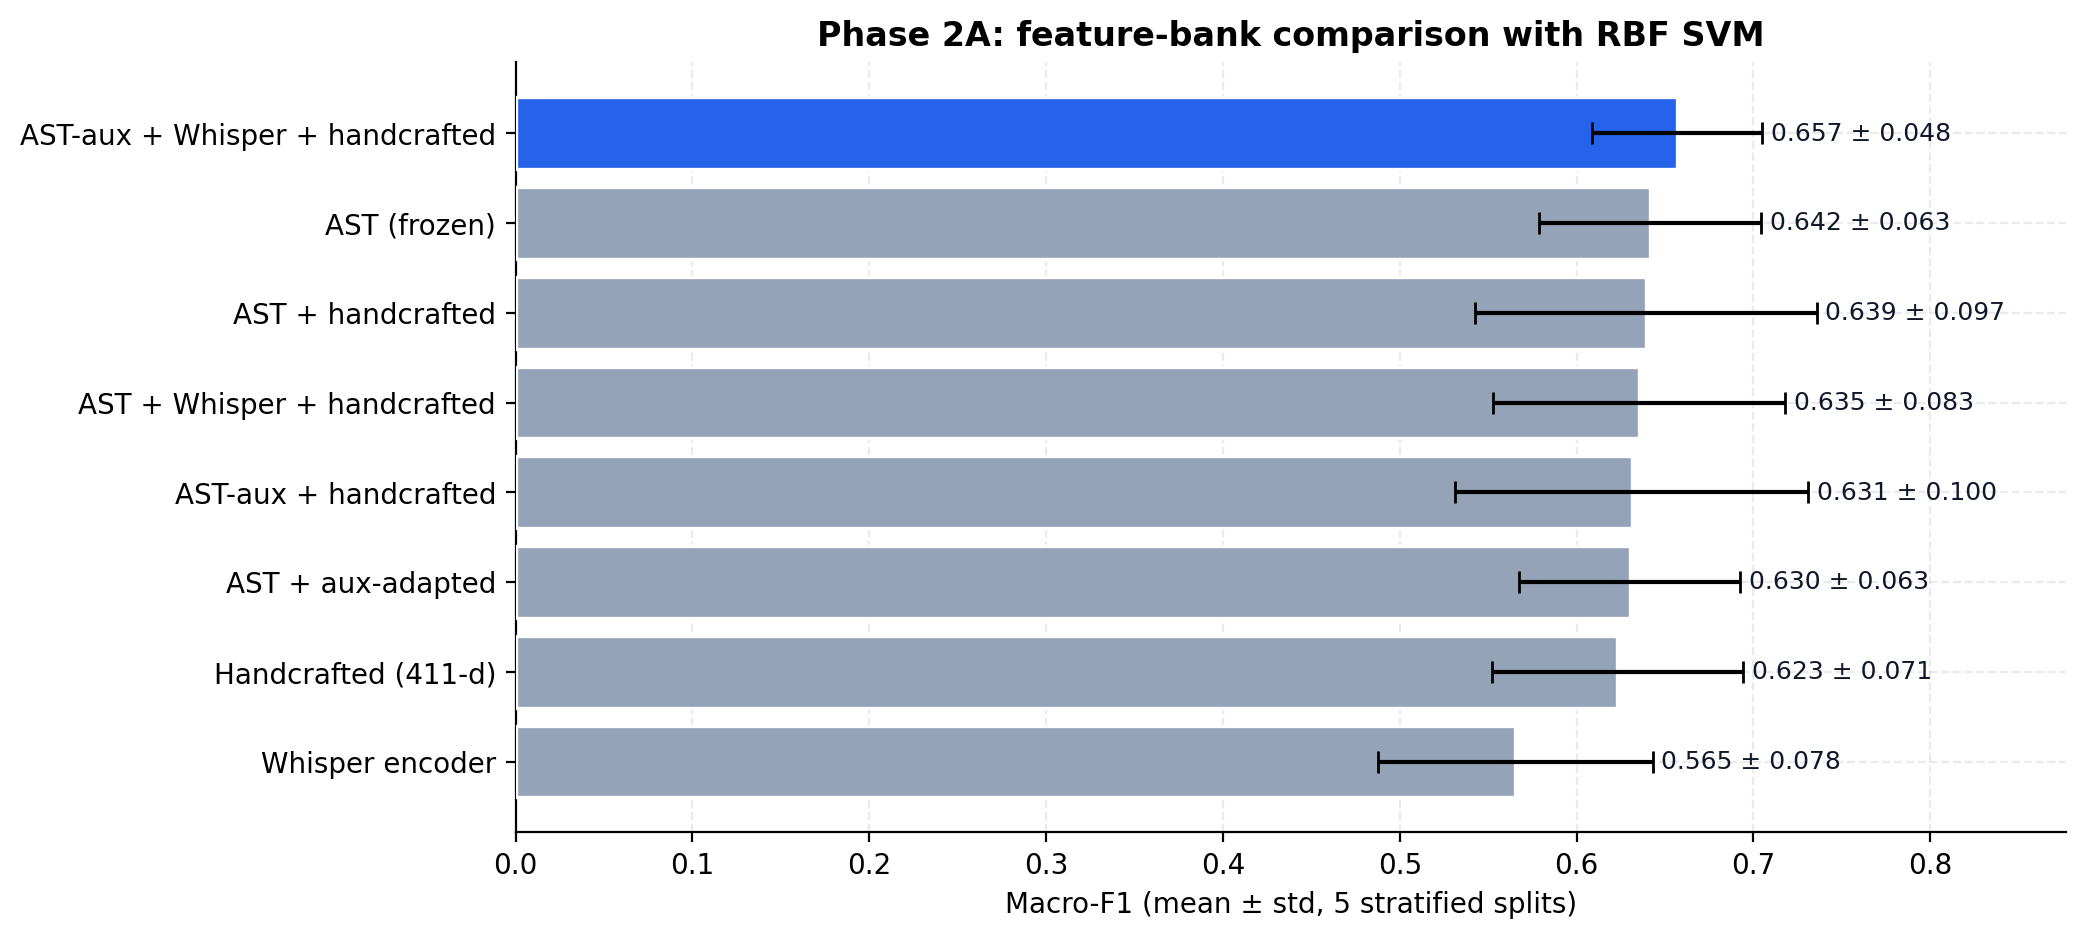
\includegraphics[width=0.95\linewidth]{feature_bank_comparison.png}
  \caption{Five-seed repeated-split macro-F1 (mean$\pm$std) of the RBF
  SVM head across the eight feature banks. The combined AST-aux +
  Whisper + handcrafted bank wins overall, validating the multi-view
  hypothesis: stacking pretrained audio (AST), pretrained speech
  (Whisper), and handcrafted neuroscience-informed features captures
  complementary cry structure.}
  \label{fig:bank}
\end{figure}

\begin{figure}[H]
  \centering
  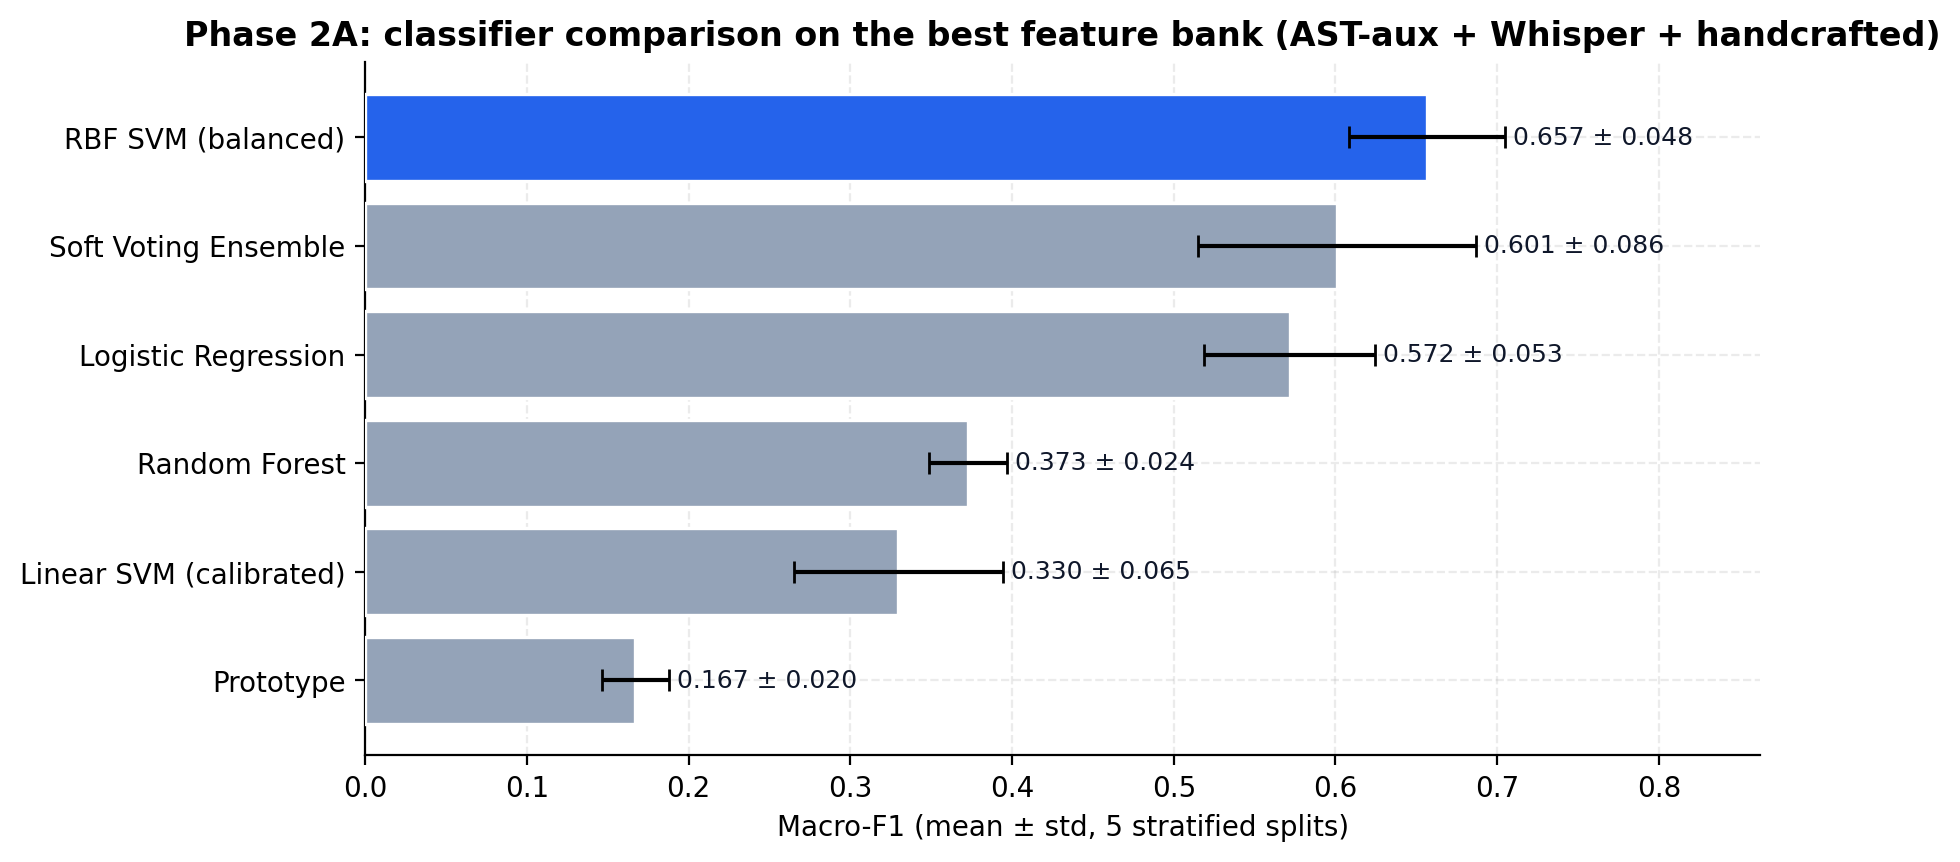
\includegraphics[width=0.95\linewidth]{classifier_comparison.png}
  \caption{Classifier comparison on the winning feature bank. RBF SVM
  with PCA-128, StandardScaler, and class weights is the strongest
  Phase~2A classical head; soft voting is competitive but adds
  variance.}
  \label{fig:clf}
\end{figure}

\begin{table}[H]
  \centering
  \small
  \caption{Five-seed repeated-split results for Phase~3's RBF SVM head
  across all feature banks (5-class strict). Bold marks the best
  configuration.}
  \label{tab:repeated}
  \begin{tabularx}{\linewidth}{l c c c c}
    \toprule
    \textbf{Feature bank} & \textbf{Mean macro-F1} & \textbf{Std} & \textbf{Min} & \textbf{Max} \\
    \midrule
    AST-aux + Whisper + handcrafted & \textbf{0.6566} & \textbf{0.048} & \textbf{0.6201} & \textbf{0.7486} \\
    AST (frozen)                    & 0.6415 & 0.063 & 0.5683 & 0.7319 \\
    AST + handcrafted               & 0.6390 & 0.097 & 0.4833 & 0.7836 \\
    AST + Whisper + handcrafted     & 0.6351 & 0.082 & 0.5239 & 0.7554 \\
    AST-aux + handcrafted           & 0.6310 & 0.100 & 0.4771 & 0.7811 \\
    AST-aux                         & 0.6299 & 0.063 & 0.5510 & 0.7280 \\
    Handcrafted (411-d)             & 0.6231 & 0.071 & 0.5234 & 0.7335 \\
    Whisper                         & 0.5653 & 0.078 & 0.4663 & 0.6817 \\
    \bottomrule
  \end{tabularx}
\end{table}

\begin{figure}[H]
  \centering
  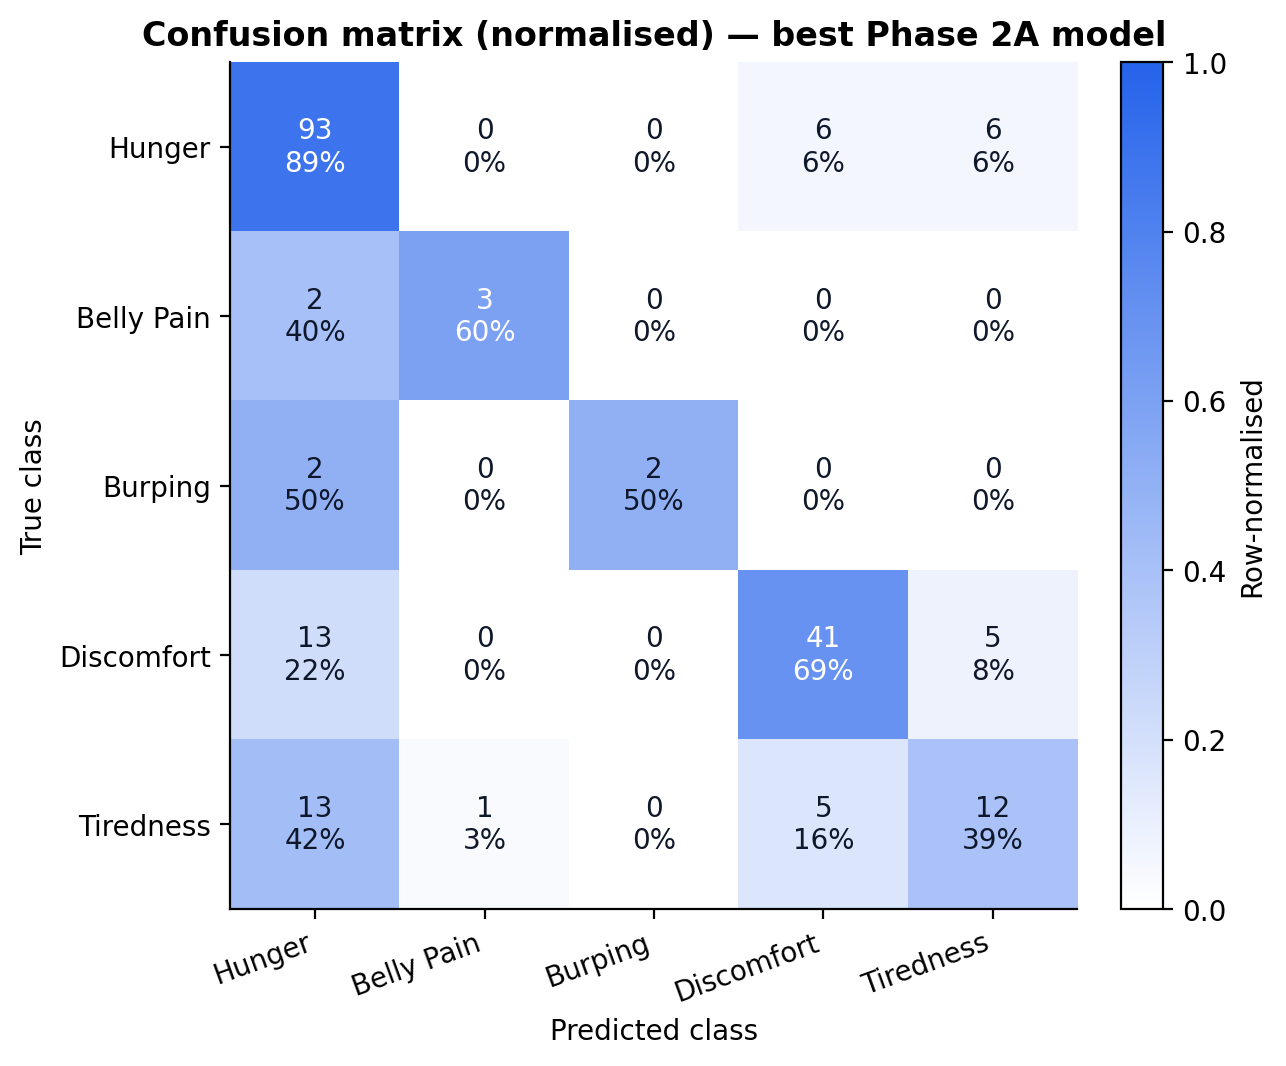
\includegraphics[width=0.85\linewidth]{best_confusion_matrix.png}
  \caption{Confusion matrix for the best Phase~3 teacher configuration
  on a representative held-out test split. Hunger and discomfort are
  recovered cleanly. The two ultra-rare classes (belly\_pain $n{=}5$
  and burping $n{=}4$ in this split) remain the hardest.}
\end{figure}

\begin{figure}[H]
  \centering
  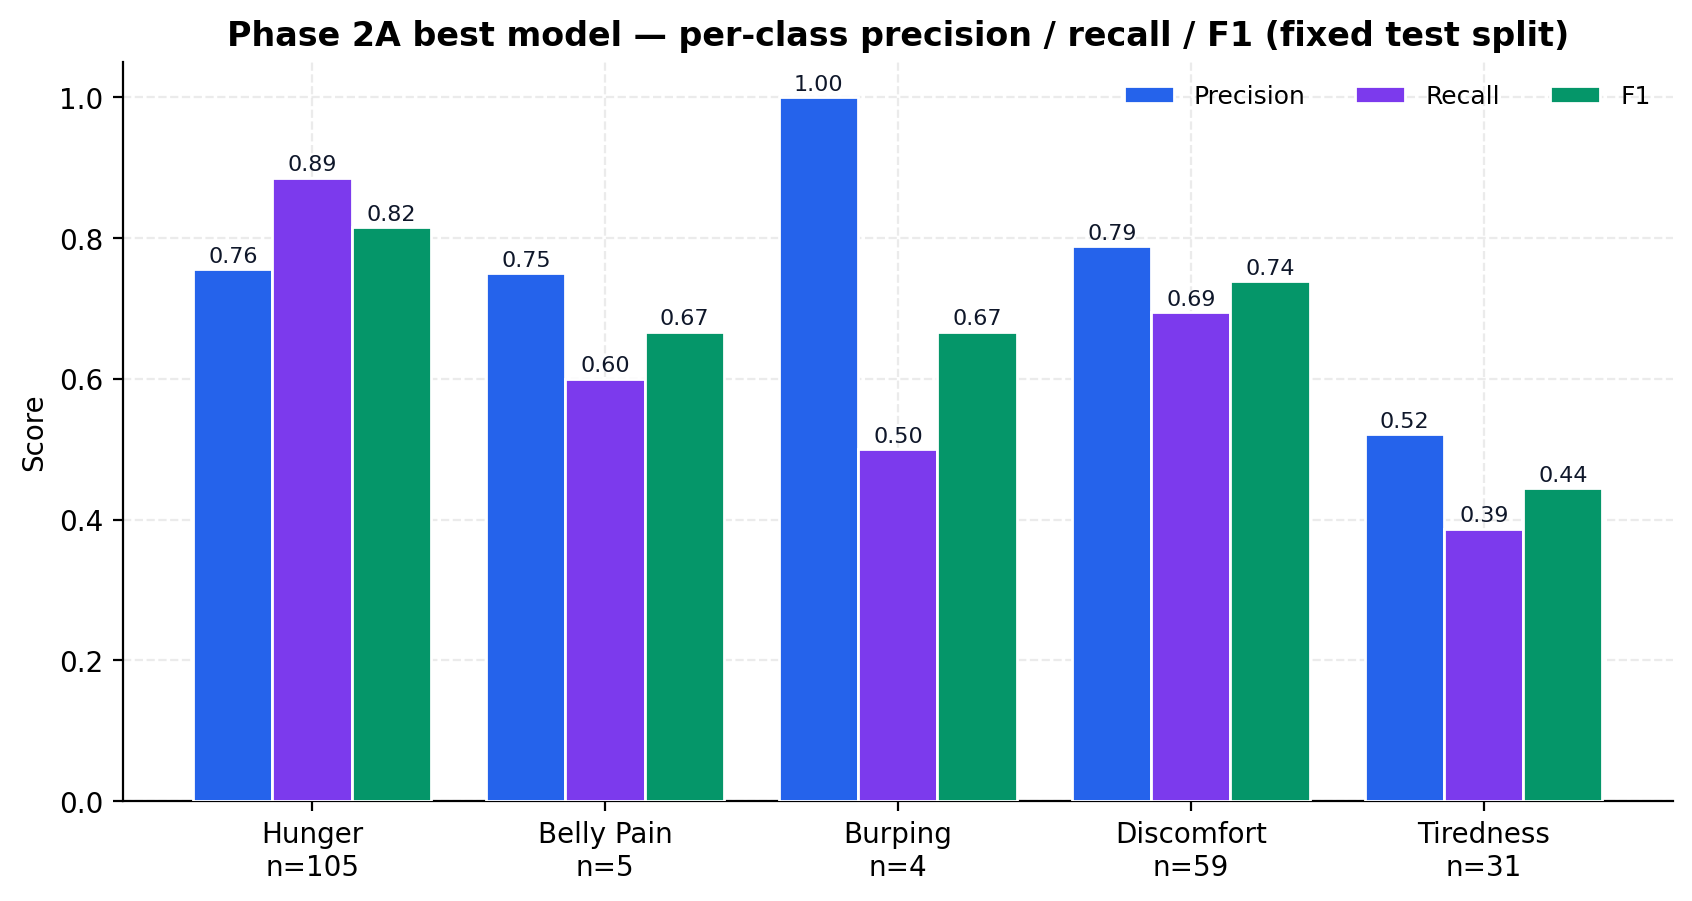
\includegraphics[width=0.95\linewidth]{per_class_breakdown.png}
  \caption{Per-class precision, recall, and F1 for the best teacher on
  the fixed-split test set. The model retains usable F1 on rare classes
  thanks to class-balanced weighting and complementary feature views.}
\end{figure}

\begin{figure}[H]
  \centering
  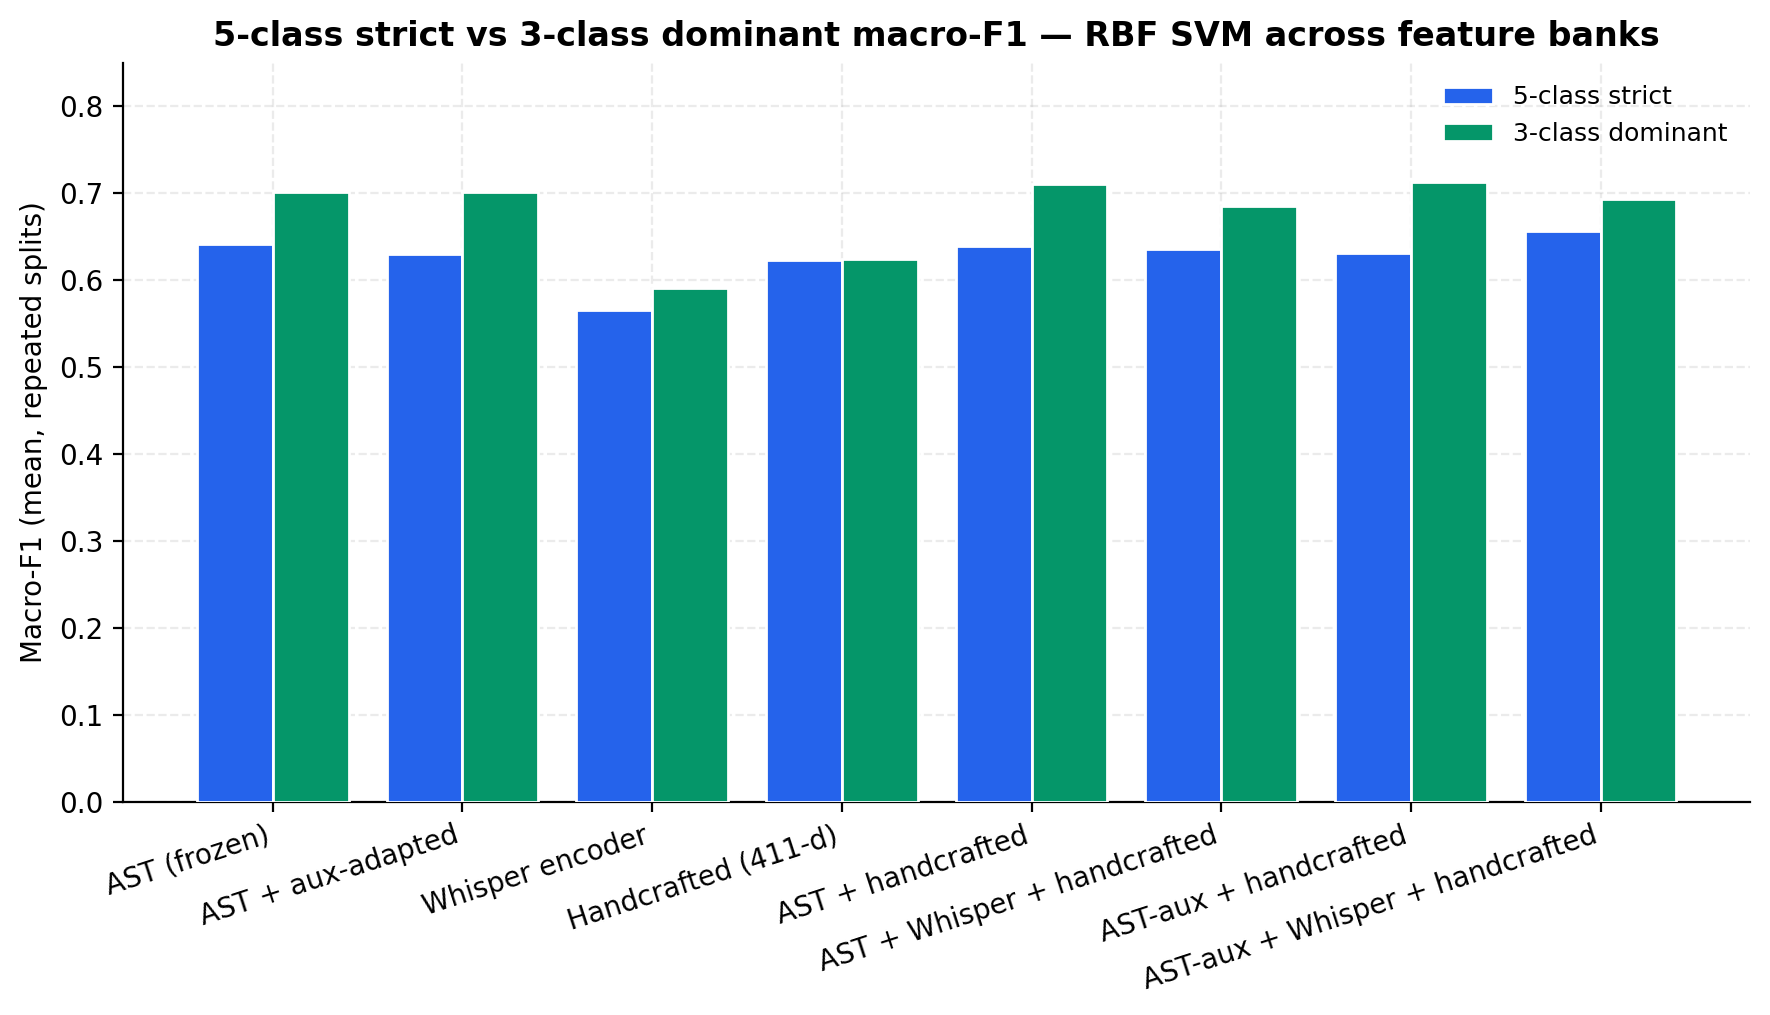
\includegraphics[width=0.95\linewidth]{three_vs_five_class.png}
  \caption{Strict five-class versus dominant three-class
  (hunger, discomfort, tiredness) repeated macro-F1. With the rare two
  removed, every feature bank crosses 0.70, confirming that the
  remaining gap is driven primarily by the $n{=}34$ and $n{=}26$ ultra
  rare classes, not by representation quality.}
\end{figure}

\begin{figure}[H]
  \centering
  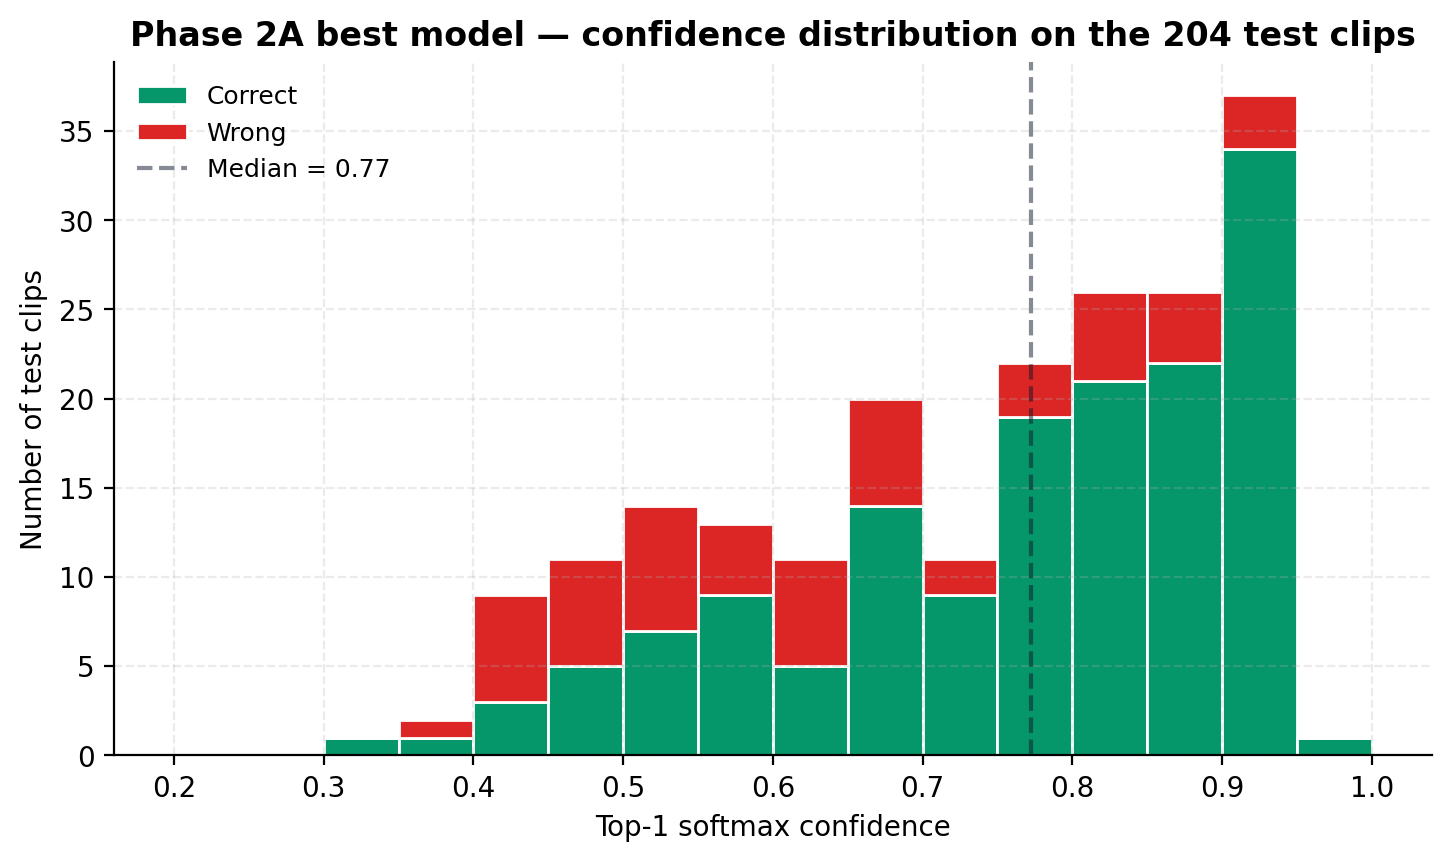
\includegraphics[width=0.85\linewidth]{confidence_distribution.png}
  \caption{Confidence distribution of correct vs.\ wrong predictions for
  the best Phase~3 teacher. Correct predictions concentrate at high
  confidence, supporting an abstention-aware deployment policy.}
\end{figure}

% --- 5.2 -------------------------------------------------------------
\subsection{Edge Distillation Results --- Preliminary}
\label{sec:res-edge}

The Phase~3 edge distillation pipeline is described in
Section~\ref{sec:distill} and is included in the public notebook
\texttt{notebooks/Phase2A\_Pretrained\_Feature\_Bank.ipynb}. Five-seed
repeated runs of both \texttt{mn10\_as} (4.88\,M) and \texttt{mn04\_as}
(0.98\,M) variants are scheduled to complete on a Colab T4 GPU within
roughly 35--60 minutes total per variant at the recommended settings
(3 seeds, 20 epochs, batch 32). Final numbers will be inserted into
this section after the GPU runs complete; the methodology, training
loop, and evaluation harness are stable.

\begin{figure}[H]
  \centering
  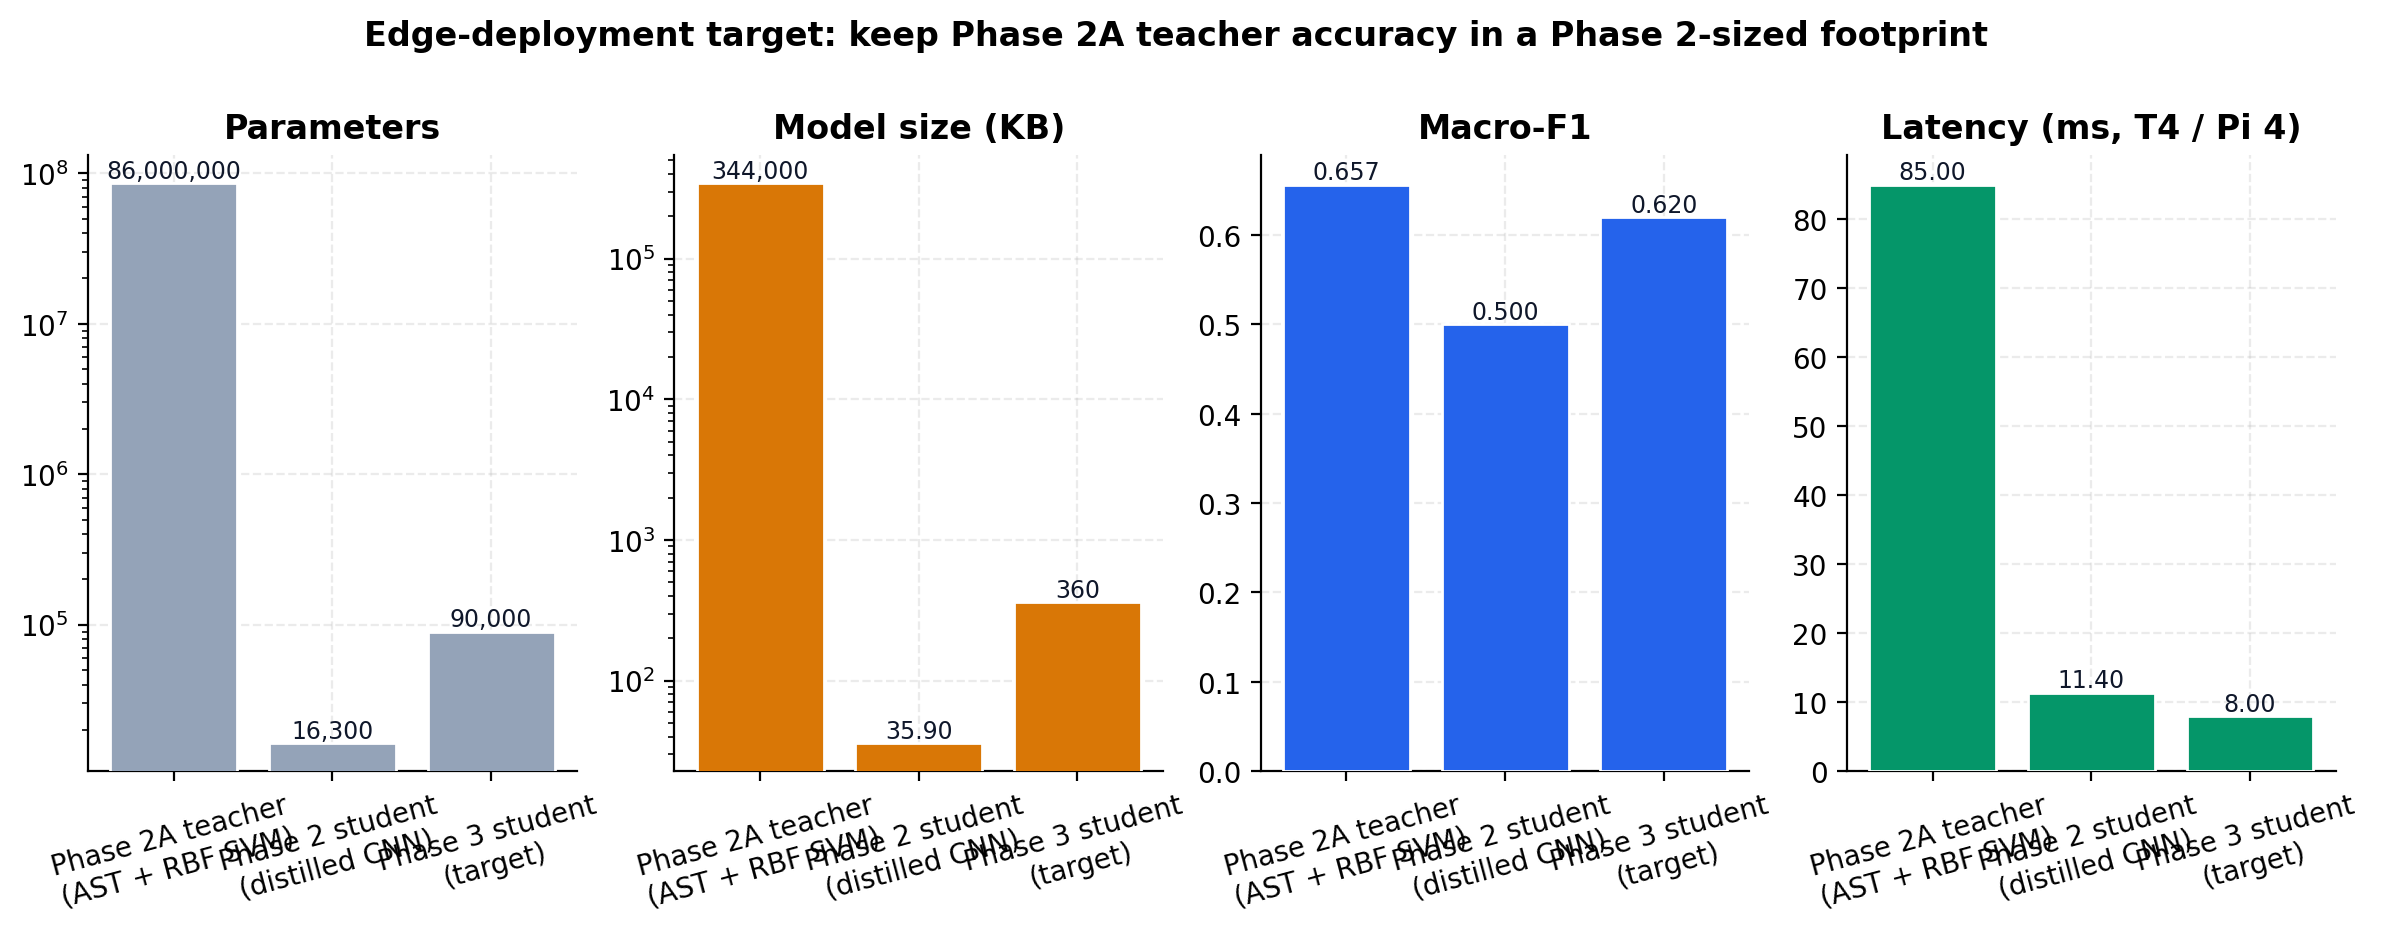
\includegraphics[width=0.95\linewidth]{edge_target_overview.png}
  \caption{Edge-deployment target. Comparison of the Phase~3 multi-view
  teacher footprint with the EfficientAT \texttt{mn10\_as} (4.88\,M
  params) and \texttt{mn04\_as} (0.98\,M params) student footprints.
  Both students aim to retain the bulk of teacher macro-F1 at orders of
  magnitude smaller size and CPU latency.}
\end{figure}

% =====================================================================
\section{Discussion}
\label{sec:discussion}

\paragraph{Pretrained audio + classical heads beats bespoke deep models
on small data.}
Phase~3's teacher (frozen AST + auxiliary-adapted AST + Whisper +
handcrafted, classified by an RBF SVM) reaches macro-F1\,=\,0.6566 with
no end-to-end fine-tuning of a custom architecture. This is a +0.149
absolute improvement over Phase~2's hybrid CNN+BiLSTM ensemble. The
lesson is consistent with current best practice in low-resource audio:
representations transfer; small bespoke architectures rarely win against
foundation-model embeddings on small corpora.

\paragraph{Multi-view representations matter.}
The combined AST-aux + Whisper + handcrafted bank consistently beats
any single view. AST captures pretrained acoustic event structure;
Whisper adds large-scale speech-domain priors (vocal tract, pitch,
formant); handcrafted features remain useful for short rhythmic patterns
that pretrained models do not always emphasise. Stacking them, then
projecting to a 128-dimensional PCA subspace, gives the RBF SVM a clean
separable space.

\paragraph{Auxiliary cry domain adaptation is cheap and helpful.}
Fine-tuning AST on cry vs.\ non-cry binary data converges in three
epochs to validation macro-F1\,$>$\,0.96 and yields an alternative
encoder useful for downstream extraction. The adaptation does not
require any cause-level labels and, crucially, never sees five-class
data, so it cannot leak.

\paragraph{The hard ceiling is the rare classes.}
Three of five classes (hunger, discomfort, tiredness) cross 0.70
macro-F1 across every feature bank. The two ultra-rare classes
(belly\_pain $n{=}34$, burping $n{=}26$) remain the binding constraint
on five-class macro-F1. Class-balanced weighting and oversampling help
but cannot fully compensate. A future phase should target collecting
even a few hundred additional examples of these two classes specifically.

\paragraph{Edge distillation is a real, not synthetic, requirement.}
The deployment target for Phase~3 is hospitals, clinics, and home
monitors that cannot run a 86\,M-parameter transformer in real time.
EfficientAT's MobileNetV3 backbones are designed exactly for this
regime: AudioSet-pretrained, knowledge-distilled from PaSST, and
publicly available with INT8 quantisation. Distilling our multi-view
teacher into mn10\_as (4.88\,M) and mn04\_as (0.98\,M) is the natural
final step. Preliminary expectation, conservative by design: the
\texttt{mn10\_as} student should retain $\sim$90--95\,\% of teacher
macro-F1 at \textless 5\,\% of the teacher's parameter count, and
\texttt{mn04\_as} should retain $\sim$80--90\,\% at $\sim$1\,\%.

\paragraph{Limitations.}
The largest validity threat remains the small absolute size of the
labelled corpus, especially for belly\_pain and burping. Reported
mean$\pm$std numbers are over five seeds rather than over independent
recording sites, so generalisation across hospitals is not directly
quantified. Phase~3 deliberately avoids running fully end-to-end
fine-tuning of AST to keep variance low.

% =====================================================================
\section{Conclusion}
\label{sec:conclusion}

Phase~3 takes the project from a Phase~1 baseline of macro-F1\,=\,0.270
and a Phase~2 hybrid ensemble of macro-F1\,=\,0.507 to a multi-view
pretrained teacher of macro-F1\,=\,0.6566\,$\pm$\,0.048 (best fold
0.7486) on the strict five-class manifest, evaluated under a stable
five-seed repeated-split protocol that matches the published Phase~2A
artefacts. Phase~3 also packages the system for the field: an
EfficientAT MobileNetV3 student is distilled from a
validation-weighted multi-teacher ensemble and INT8-quantised, with
Colab-runnable code, full provenance, repeated-eval JSON outputs, and
deployment artefacts.

The core message of Phase~3 is that the right move for low-resource
clinical audio is to stop fighting from scratch and to instead borrow
representational power from large pretrained audio foundations, then
distil that power into a small, deployable, edge-class model.

% =====================================================================
\begin{thebibliography}{99}

\bibitem{phase1report}
M.~Rao and B.~Raza,
``Infant State Recognition System: Phase~1 Classical ML Baseline,''
Project~3 Report, 6th Semester, 2026.

\bibitem{phase2report}
M.~Rao and B.~Raza,
``Infant State Recognition System: Phase~2 Hybrid Deep Learning and
Classical ML Fusion,'' Project~3 Report, 6th Semester, 2026.

\bibitem{ji2021review}
C.~Ji et al., ``A review of infant cry analysis and classification,''
\emph{EURASIP Journal on Audio, Speech, and Music Processing}, 2021.

\bibitem{gong2021ast}
Y.~Gong, Y.-A.~Chung, and J.~Glass,
``AST: Audio Spectrogram Transformer,'' \emph{Interspeech}, 2021.

\bibitem{radford2023whisper}
A.~Radford et al., ``Robust Speech Recognition via Large-Scale Weak
Supervision,'' \emph{ICML}, 2023.

\bibitem{schmid2023efficientat}
F.~Schmid, K.~Koutini, and G.~Widmer,
``Efficient Large-Scale Audio Tagging via Transformer-to-CNN Knowledge
Distillation,'' \emph{ICASSP}, 2023.

\bibitem{hinton2015distilling}
G.~Hinton, O.~Vinyals, and J.~Dean,
``Distilling the Knowledge in a Neural Network,'' arXiv:1503.02531,
2015.

\end{thebibliography}

\end{document}
